\documentclass[10pt]{article}
\usepackage[a4paper, margin=2cm]{geometry}
%\usepackage{fullpage}
\usepackage[T1]{fontenc}
\usepackage[utf8]{inputenc}
\usepackage{graphicx}
\usepackage{mathpazo}
\pagenumbering{arabic}
\usepackage{siunitx}
\usepackage{amsmath}
\usepackage{mathtools} % Para poder usar "\Aboxed"
\usepackage{cancel} % Para usar "\cancel", de https://tex.stackexchange.com/questions/537955/how-do-cross-out-text-in-math-mode
\usepackage{multicol}
\usepackage[spanish]{babel}
\usepackage{steinmetz}
\DeclareSIUnit\voltampere{VA}
\DeclareSIUnit\var{VAr}
\setlength\parindent{0pt} % no indent

% Numbering pages on the right footer:
% (https://tex.stackexchange.com/questions/153167/how-to-set-page-number-at-right-footer)
\usepackage{fancyhdr}
% Turn on the style
\pagestyle{fancy}
\fancyhf{} % sets both header and footer to nothing
\renewcommand{\headrulewidth}{0pt} % To remove the top horizontal line created by default by "fancyhdr", from here: https://tex.stackexchange.com/questions/13896/how-to-remove-the-top-horizontal-bar-in-fancyhdr
% Set the right side of the footer to be the page number
\fancyfoot[R]{\thepage}


\usepackage{minibox} % Para poder partir el texto en 2 líneas usando "underbrace" u "overbrace", info aquí: https://tex.stackexchange.com/questions/8680/how-can-i-insert-a-newline-in-a-framebox


\usepackage{xparse} % For "overbrace/underbrace but with an arrow instead", from https://tex.stackexchange.com/questions/8720/overbrace-underbrace-but-with-an-arrow-instead

% Para poner flechas sobre los signos de igual, de aquí: https://tex.stackexchange.com/questions/8720/overbrace-underbrace-but-with-an-arrow-instead
\NewDocumentCommand{\overarrow}{O{=} O{\uparrow} m}{%
  \overset{\makebox[0pt]{\begin{tabular}{@{}c@{}}#3\\[0pt]\ensuremath{#2}\end{tabular}}}{#1}
}
\NewDocumentCommand{\underarrow}{O{=} O{\downarrow} m}{%
  \underset{\makebox[0pt]{\begin{tabular}{@{}c@{}}\ensuremath{#2}\\[0pt]#3\end{tabular}}}{#1}
}



\begin{document}

\large{\textbf{Ejercicio 10 de la colección de problemas}}

\vspace{3mm}
\large{\textbf{Enunciado}}:

\vspace{5mm}

En el circuito de la figura, determinar:
\begin{enumerate}
    \item Las ecuaciones para el cálculo de las intensidades
    \item Todas las intensidades indicadas
    \item Potenciales en todos los nudos
    \item Carga y energía almacenada en los condensadores
\end{enumerate}

\begin{minipage}{0.85\linewidth}
  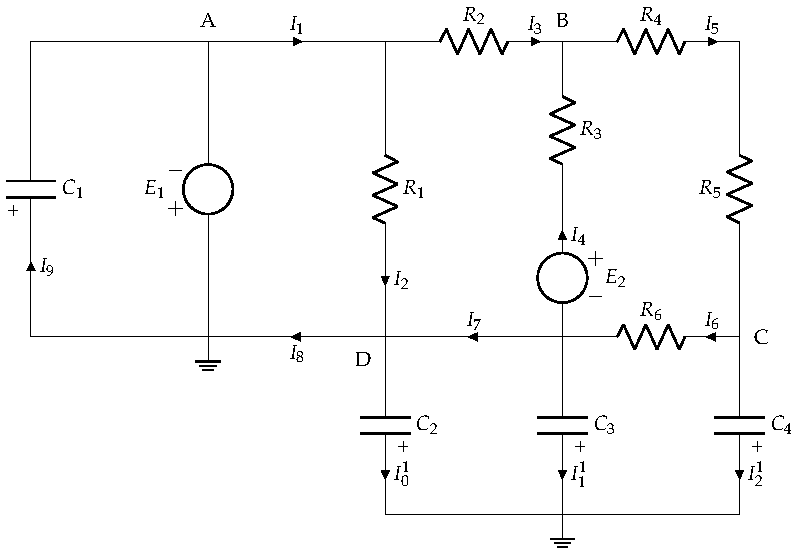
\includegraphics[scale=1.1]{figs/BT1_11.pdf}
\end{minipage}
\hfill
\begin{minipage}{0.11\linewidth}
    \vspace{-40mm}
    
    \textbf{Datos}:
    \vspace{2mm}
    
    $R_1 = \qty{2}{\ohm}$\\
    $R_2 = \qty{4}{\ohm}$\\
    $R_3 = \qty{2}{\ohm}$\\
    $R_4 = \qty{1}{\ohm}$\\
    $R_5 = \qty{2}{\ohm}$\\
    $R_6 = \qty{1}{\ohm}$\\
    $C_i = \qty[parse-numbers=false]{i}{\micro\farad}$\\
    $E_1=\qty{8}{\volt}$\\
    $E_2 = \qty{8}{\volt}$   
\end{minipage}

\vspace{3mm}

\hrulefill

\vspace{5mm}
\textbf{Solución}:
\vspace{4mm}

Al tratarse de alimentación en CC, se sustituyen los condensadores por circuitos abiertos, quedando el circuito de la figura (ver página siguiente).

\vspace{7mm}
Aplicando el método de mallas, con las corrientes indicadas, se plantea el sistema de ecuaciones en forma matricial:
\begin{equation*}
  \begin{bmatrix}
    2 & -2 & 0 \\
    -2 & 8 & -2 \\
    0 & -2 & 6
  \end{bmatrix} \cdot
  \begin{bmatrix}
    I_a\\
    I_b\\
    I_c
  \end{bmatrix} = %
  \begin{bmatrix}
    -8 \\
    -8\\
    8
  \end{bmatrix}
\end{equation*}

\vspace{2mm}
Las ecuaciones completas para calcular las intensidades son:
\begin{align*}
  2\,I_a&-2\,I_b = -8\\
  -2\,I_a&+8\,I_b-2\,I_c = -8\\
  -2\,I_b&+ 6\,I_c = 8
\end{align*}

\newpage

Cuya solución es:

\vspace{-8mm}
\begin{align*}
  I_a&=\qty{-6.5}{\ampere}\\
  I_b&=\qty{-2.5}{\ampere}\\
  I_c&=\qty{0.5}{\ampere}\\
\end{align*}

\vspace{-10mm}
\begin{center}
  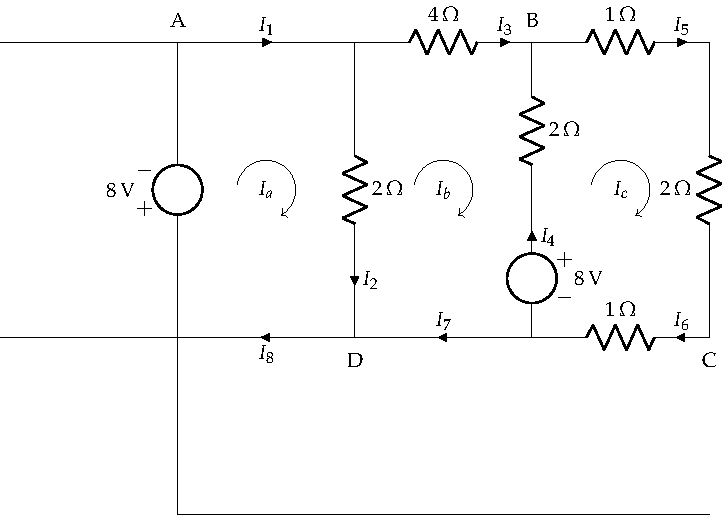
\includegraphics[scale=1.1]{figs/BT1_11_mod.pdf}
\end{center}

\vspace{2mm}
Estableciendo las relaciones entre las corrientes de malla y las de rama del circuito:
\begin{align*}
  I_1&=I_8=I_a= \boxed{\qty{-6.5}{\ampere}}\\
  I_2&=I_a-I_b=-6.5-(-2.5)= \boxed{\qty{-4}{\ampere}}\\
  I_3&=I_7=I_b= \boxed{\qty{-2.5}{\ampere}}\\
  I_4&=I_c-I_b=0.5-(-2.5)= \boxed{\qty{3}{\ampere}}\\
  I_5&=I_6=I_c= \boxed{\qty{0.5}{\ampere}}\\
\end{align*}

\vspace{-2mm}
Una forma alternativa de resolver el circuito consiste en reparar en que $E_1$ es generador dominante, por lo que puede determinarse directamente el valor de $I_2 = - E_1 / R_1 = -4\si{\ampere}$. Esto permite usar únicamente 2 mallas, lo que reduce el sistema de ecuaciones a $2\times 2$: 

\vspace{4mm}
\begin{minipage}{0.6\linewidth}
    \begin{center}
    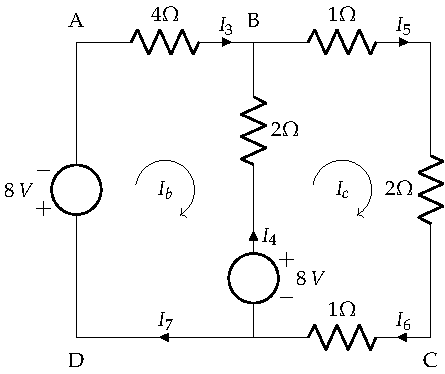
\includegraphics[scale=1.1]{figs/BT1_11_mod2.pdf}
    \end{center}
\end{minipage}
\begin{minipage}{0.4\linewidth}
    \begin{equation*}
      \begin{bmatrix}
        6 & -2  \\
        -2 & 6
      \end{bmatrix} \cdot
      \begin{bmatrix}
        I_b\\
        I_c
      \end{bmatrix} = %
      \begin{bmatrix}
        -16\\
        8
      \end{bmatrix}
    \end{equation*}

    \vspace{10mm}
    
    Cuya solución es la misma que 
    
    la obtenida anteriormente.
\end{minipage}

Conociendo las corrientes y teniendo el nudo de tierra como referencia, se calculan los potenciales:
\begin{align*}
  U_A&=-U_{8V}= \boxed{\qty{-8}{\volt}}\\
  U_B&=-U_{R2\Omega}+U_{8V}=-2\cdot 3+8= \boxed{\qty{2}{\volt}}\\
  U_C&=U_{R1\Omega}=1\cdot 0.5= \boxed{\qty{0.5}{\volt}}\\
  U_D&= \boxed{\qty{0}{\volt}}
\end{align*}

\vspace{4mm}
Con los potenciales, se determina la carga de los condensadores:
\begin{align*}
  Q_{1\mu F}&=C_{1\mu F}\, (-U_{A}) = 1\cdot 10^{-6}\cdot (-(-8))= \boxed{\qty{8}{\micro\coulomb}}\\
  Q_{2\mu F}&=C_{2\mu F} \cdot \qty{0}{\volt} = \boxed{\qty{0}{\micro\coulomb}}\\
  Q_{3\mu F}&=C_{3\mu F} \cdot \qty{0}{\volt} = \boxed{\qty{0}{\micro\coulomb}}\\
  Q_{4\mu F}&=C_{4\mu F}\, (-U_C) = 4\cdot 10^{-6}\cdot (-0.5)= \boxed{\qty{-2}{\micro\coulomb}}
\end{align*}

\vspace{4mm}
Aquellos condensadores en los que la carga es negativa, significa que tienen polaridad contraria a la considerada. La energía almacenada en cada uno de ellos es:

\begin{align*}
  E_{1\mu F}&=\dfrac{1}{2}\,C_{1\mu F}\cdot (-U_{A})^2 = \dfrac{1}{2}\cdot 1\cdot 10^{-6}\cdot (-(-8))^2= \boxed{\qty{32}{\micro\joule}}\\
  E_{2\mu F}&= \boxed{\qty{0}{\micro\joule}}\\
  E_{3\mu F}&= \boxed{\qty{0}{\micro\joule}}\\
  E_{4\mu F}&=\dfrac{1}{2}\,C_{4\mu F}\cdot (-U_{C})^2 = \dfrac{1}{2}\cdot 4\cdot 10^{-6}\cdot (-0.5)^2= \boxed{\qty{0.5}{\micro\joule}}
\end{align*}


\end{document}
